\documentclass{beamer}
\usepackage{graphicx}
\graphicspath{ {images/} }
\usepackage{float}
\usepackage{wrapfig}
\usepackage{pstricks}

%\usetheme{Goettingen}
%\usetheme{Berkeley}
%\usetheme{Boadilla}
\usetheme{Warsaw}

\usepackage[utf8]{inputenc}
\usepackage[spanish]{babel}

%%%%%%%%%%%%%%%%%%%%%%%%%%%%%%%%%%%%%%%%%%%%%%%%%%%%%%
%%%%%%%%%%%%%%%%%%%%%%%%%%%%%%%%%%%%%%%%%%%%%%%%%%%%%%
%% INFORMACION GENERAL
%%%%%%%%%%%%%%%%%%%%%%%%%%%%%%%%%%%%%%%%%%%%%%%%%%%%%%
%%%%%%%%%%%%%%%%%%%%%%%%%%%%%%%%%%%%%%%%%%%%%%%%%%%%%%
\title[Charla Android]{Android Invaders}
\author[LPB]{$@asolisi, @juanvelascogomez y @neon520$}
\institute[UGR]{Universidad de Granada}

\begin{document}

\maketitle

%los comandos con asterisco evitan la numeración
\section*{Introducción}
\begin{frame}
	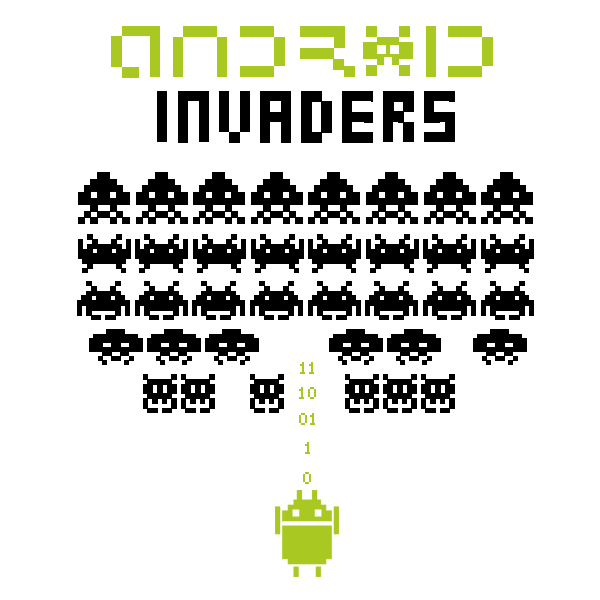
\includegraphics[width=10cm, height=7cm]{androidInvaders_nobackground_black.png}
\end{frame}

%%%%%%%%%%%%%%%%%%%%%%%%%%%%%%%%%%%%%%%%%%%%%%%%%%%%%%
%%%%%%%%%%%%%%%%%%%%%%%%%%%%%%%%%%%%%%%%%%%%%%%%%%%%%%
%% Primera parte: Introduccion
%%%%%%%%%%%%%%%%%%%%%%%%%%%%%%%%%%%%%%%%%%%%%%%%%%%%%%
%%%%%%%%%%%%%%%%%%%%%%%%%%%%%%%%%%%%%%%%%%%%%%%%%%%%%%
\begin{frame}{¿Dónde está el problema?}
	\begin{itemize}[<+-|alert@+>]
		
	\item Los dispositivos y entornos móviles son un objetivo y están constantemente amenazados por:
	\item Comportamientos del usuario arriesgados (y habituales)
	\item Vulnerabilidades de seguridad
	\item Dar a las actualizaciones la importancia que se merecen
	
	\end{itemize}
\end{frame}

%Segundo grupo: Actualizaciones del sistema
\begin{frame}{Actualizaciones del sistema}
	Algunas preguntas a resolver...
	
\begin{itemize}[<+-|alert@+>]
	
	\item ¿Disponéis de la última versión del sistema operativo para vuestro móvil?
	\item ¿Está disponible esa nueva versión para nuestro dispositivo?
	\item ¿Resuelve esto todas las vulnerabilidades conocidas?
	\item ¿Y las que no son públicas?
	
\end{itemize}
\end{frame}

%Tercer grupo: Vulnerabilidades Android
\begin{frame}{Versiones y vulnerabilidades en Android}
	
	\begin{block}{Android: 8 años}
		2008: 1.0
		
		2009: 1.1, 1.5, 1.6, 2.0
		
		2010: 2.1, 2.2, 2.3.x
		
		2011: 2.4.x, 3.x,4.0
		
		2012: 4.1, 4.2
		
		2013: 4.3, 4.4
		
		2014: 5.0
		
		2015: 5.1, 6.0
	\end{block}
		
\end{frame}

%Cuarto grupo: Vulnerabilidades Android II
\begin{frame}{Versiones y vulnerabilidades en Android}
	
	\begin{alertblock}{Número oficial de vulnerabilidades}
		
		Desconocido (hasta Agosto 2015 para móviles Nexus)
		
		\begin{itemize}[<+-|alert@+>]
			
			\item Agosto de 2015: 6
			\item Septiembre de 2015: 9
			\item Octubre de 2015: 30
			\item Noviembre de 2015: 7
			\item TOTAL: 52 vulnerabilidades conocidas
			
		\end{itemize}
	\end{alertblock}
	
\end{frame}

%Cuarto grupo: Usuarios y contraseñas
\begin{frame}{Sobre los usuarios y contraseñas}
	
	\begin{itemize}[<+-|alert@+>]
		
		\item \textbf{¿Tenéis cuenta de usuario en la plataforma del fabricante del dispositivo móvil?}
		\item \textbf{¿Vuestro usuario es conocido?}
		\item ¿Seguro?
		\item \textbf{¿La contraseña es robusta?}
		\item ¿La reutilizáis?
		
	\begin{block}{TOP de contraseñas más usadas en 2015}
		123456
		
		password
		
		12345678
		
		qwerty
		
		iloveyou
		
	\end{block}
	
	\end{itemize}
	
\end{frame}


%%%%%%%%%%%%%%%%%%%%%%%%%%%%%%%%%%%%%%%%%%%%%%%%%%%%%%
%%%%%%%%%%%%%%%%%%%%%%%%%%%%%%%%%%%%%%%%%%%%%%%%%%%%%%
%% Segunda parte: Camuflar un APK
%%%%%%%%%%%%%%%%%%%%%%%%%%%%%%%%%%%%%%%%%%%%%%%%%%%%%%
%%%%%%%%%%%%%%%%%%%%%%%%%%%%%%%%%%%%%%%%%%%%%%%%%%%%%%
\section{Camuflar un APK}

\begin{frame}{Otra cosa mariposa}

Trabajando en ello...

\end{frame}


%%%%%%%%%%%%%%%%%%%%%%%%%%%%%%%%%%%%%%%%%%%%%%%%%%%%%%
%%%%%%%%%%%%%%%%%%%%%%%%%%%%%%%%%%%%%%%%%%%%%%%%%%%%%%
%% Tercera parte: Prueba de concepto
%%%%%%%%%%%%%%%%%%%%%%%%%%%%%%%%%%%%%%%%%%%%%%%%%%%%%%
%%%%%%%%%%%%%%%%%%%%%%%%%%%%%%%%%%%%%%%%%%%%%%%%%%%%%%
\section{Prueba de concepto. Intrusión en dispositivo}

\begin{frame}

\centering Prueba de concepto


\includegraphics[width=5cm, height=7cm]{poc.jpg}

\end{frame}


%%%%%%%%%%%%%%%%%%%%%%%%%%%%%%%%%%%%%%%%%%%%%%%%%%%%%%
%%%%%%%%%%%%%%%%%%%%%%%%%%%%%%%%%%%%%%%%%%%%%%%%%%%%%%
%% Cuarta parte: Ataques fuera de LAN
%%%%%%%%%%%%%%%%%%%%%%%%%%%%%%%%%%%%%%%%%%%%%%%%%%%%%%
%%%%%%%%%%%%%%%%%%%%%%%%%%%%%%%%%%%%%%%%%%%%%%%%%%%%%%

\section{¿Y si salimos afuera?}

\subsection{Impresiones}

\begin{frame}{Últimas notas y títulos}

Trabajando en ello...

\end{frame}

%%%%%%%%%%%%%%%%%%%%%%%%%%%%%%%%%%%%%%%%%%%%%%%%%%%%%%
%%%%%%%%%%%%%%%%%%%%%%%%%%%%%%%%%%%%%%%%%%%%%%%%%%%%%%
%% Bibliografia
%%%%%%%%%%%%%%%%%%%%%%%%%%%%%%%%%%%%%%%%%%%%%%%%%%%%%%
%%%%%%%%%%%%%%%%%%%%%%%%%%%%%%%%%%%%%%%%%%%%%%%%%%%%%%
\begin{thebibliography}{10}
\bibitem{lshort} Esto es la bibliografía. Pendiente de subir.
\end{thebibliography}

\end{document}
